\documentclass[a4paper, oneside]{discothesis}

\usepackage[utf8]{inputenc}
\usepackage[T1]{fontenc}
\usepackage{algpseudocode}
\usepackage{algorithm}
\usepackage{mathtools}
\usepackage{subcaption}
\usepackage{tikz}
\usepackage{hyperref}
\usepackage{minted}
\usepackage{commath}
\usetikzlibrary{arrows.meta}


%%%%%%%%%%%%%%%%%%%%%%%%%%%%%%%%%%%%%%%%%%%%%%%%%%%%%%%%%%%%%%%%%%%%%%%%%%%%%%%%%%%%%%%%%%%%%%%%%
% DOCUMENT METADATA

\thesistype{Bachelor's Thesis} % Master's Thesis, Bachelor's Thesis, Semester Thesis, Group Project
\title{Exploration of Arvy Heuristics in Sequential Distributed Mutual Exclusion}

\author{Silvan Mosberger}
\email{msilvan@student.ethz.ch}

\institute{Distributed Computing Group \\[2pt]
Computer Engineering and Networks Laboratory \\[2pt]
ETH Zürich}

\supervisors{András Papp, Pankaj Khanchandani\\[2pt] Prof.\ Dr.\ Roger Wattenhofer}

% Optionally, keywords and categories of the work can be shown (on the Abstract page)
\keywords{Arrow, Ivy, distributed directory, shared object}
\categories{Network algorithms}

\date{\today}

%%%%%%%%%%%%%%%%%%%%%%%%%%%%%%%%%%%%%%%%%%%%%%%%%%%%%%%%%%%%%%%%%%%%%%%%%%%%%%%%%%%%%%%%%%%%%%%%%

\begin{document}

\frontmatter % do not remove this line
\maketitle

\cleardoublepage

\begin{acknowledgements}
I thank my advisors Pankaj and András for the weekly discussions, which helped greatly in guiding the direction of this work and developing new ideas.
\end{acknowledgements}


\begin{abstract}
The abstract should be short, stating what you did and what the most important result is.
Lorem ipsum dolor sit amet, consetetur sadipscing elitr, sed diam nonumy eirmod tempor invidunt ut labore et dolore magna aliquyam erat, sed diam voluptua. At vero eos et accusam et justo duo dolores et ea rebum. Stet clita kasd gubergren, no sea takimata sanctus est Lorem ipsum dolor sit amet. Lorem ipsum dolor sit amet, consetetur sadipscing elitr, sed diam nonumy eirmod tempor invidunt ut labore et dolore magna aliquyam erat, sed diam voluptua. At vero eos et accusam et justo duo dolores et ea rebum. Stet clita kasd gubergren, no sea takimata sanctus est Lorem ipsum dolor sit amet.
\end{abstract}

\tableofcontents

\mainmatter

\chapter{Introduction}

Often in computing a single resource is shared between multiple components, where only one of them may access it at a time. In a distributed setting an algorithm to solve this is called a distributed mutual exclusion algorithm or distributed directory protocol. A trivial solution is to dedicate a single node to be the center where all requests for the resource should go, with the disadvantage of a lot of traffic for many concurrent requests. Better solutions to this problem include the Arrow and Ivy protocols, both of which work on similar principles to be explained in the following sections. In the Arvy paper these protocols have been combined in a flexible manner to allow a whole set of algorithms to be created while still guaranteeing correctness.

In this thesis we explore this set of Arvy algorithms with the hope of finding ones that work better than any already existing ones

\section{Model}
\label{model}

We consider a complete graph $G=(V,E)$ with $n\coloneqq|V|$ vertices and $m\coloneqq\binom{n}{2}$ edges. Each edge has a cost $c : E \rightarrow \mathbb{R}$ associated with it, representing the amount of time it takes a message to traverse it. The cost function forms a metric space:
\begin{itemize}
\item The cost from a node to itself is zero: $\forall v:c(v, v)=0$
\item Costs between different nodes are positive: $\forall u,v : u\neq v\Rightarrow c(u,v)>0$
\item Costs are the same in both directions: $\forall u,v : c(u,v)=c(v,u)$
\item Triangle inequality: $\forall u,v,w : c(u,w)\leq c(u,v)+c(v,w)$
\end{itemize}

As a reasonable constraint, a node $v$ can only query costs from itself to other nodes, so it has access to $\{c(v, u)\;|\;u\in V\}$. In a realistic scenario these costs can be obtained and updated by doing regular pings to other nodes. In our model we don't consider changing costs however.

In addition, Every node can be considered a machine with the ability to execute arbitrary effectful code such as reading/writing state or generating randomness. We model execution to be atomic, so no time passes during it. Therefore traversing graph edges are the only place to spend time on.

A major simplification we make is that nodes can only request the token in series. So only after the token has reached the requesting node another node can make a request for it. Therefore requests can be represented as an series $R=\{r_1,r_2,\dots\},r_i\in V$ where $r_i$ encodes the $i$-th request originating from node $r_i$. While this series could be endless, for being able to reason more easily about execution time we let it be finite.

In the type of algorithms we'll look at, when the $i$-th request gets made by node $r_i$, the request travels along some path $A_i=\{a_i^{(0)},a_i^{(1)},\dots,a_i^{(l_i)}\}$ with $l_i=|A_i|-1$ being the index of the last node as well as the number of messages that are being sent. Then $a_i^{(0)}=r_i$ is the node making the request and the $a_i^{(l_i)}$ is the node currently holding the token. After the request was sent along this path, the token is then sent directly from $a_i^{(l_i)}$ to $a_i^{(0)}$ to satisfy the request. Without loss of generality, nodes can't send requests when they have the token already, meaning $a_i^{(0)}\neq a_i^{(l_i)}$ or $|A_i|\geq 2$. In addition, it holds that $a_i^{(0)}=a_{i+1}^{(l_{i+1})}$ for all $i\in\mathbb{N}$, meaning the node making a request in a request will be the last node in the request path in the following request.

The goal is to satisfy the requests most efficiently. We first define $c(A_i)$ to be the cost of traversing request path $A_i$:
\begin{equation}
c(A_i)\coloneqq\sum_{k=1}^{l_i}c(a_i^{(k-1)}, a_i^{(k)})
\end{equation}

Also let $c_{avg}$ be the average cost of an edge in the graph:
\begin{equation}
c_{avg}=\frac{1}{|V|^2}\sum_{u,v\in V}c(u,v)
\end{equation}

Now there are different reasonable ways to define efficiency for a sequence of requests $R$.
\begin{itemize}
\item
  One way is to look at the average time it takes to satisfy a request. This would include the cost to traverse the request path in addition to sending the token back. However because the cost to send the token back is unchangeable in our case we ignore it. To get a measure that's independent of the cost values in the graph, we divide by $c_{avg}$ as well.
  \begin{equation}
    \mathcal{C}_{time}(R) = \frac{1}{|R|}\sum_{i=1}^{|R|}\frac{c(A_i)}{c_{avg}}
  \end{equation}

  This measure is better suited for overall performance because the occasional poorly performing request gets averaged out.
  
\item
  Another way is to look at how much worse the request paths are than a direct connection.
  \begin{equation}
    \mathcal{C}_{ratio}(R) = \frac{1}{|R|}\sum_{i=1}^{|R|}\frac{c(A_i)}{c(p_i^{(0)},p_i^{(l_i)})}
  \end{equation}

  This measure penalizes request paths that are much longer than the direct path, so it's better suited for getting a sense of how individual requests are doing.

\item
  Even though in our model there is no execution time for computations on nodes, it could still be interesting to see how many nodes a request has to travel through. Therefore we define another measure, the average hop count:
  \begin{equation}
    \mathcal{C}_{hops}(r) = \frac{1}{|R|}\sum_il_i
  \end{equation}
\end{itemize}


\section{Arrow, Ivy and Arvy}

Two well-known algorithms for solving this problem are Arrow and Ivy, which are both a special case of an Arvy algorithm, which is where its name comes from.

All of these algorithms are based on the idea of maintaining a rooted spanning tree over time: Every node stores a pointer to its parent $parent : V \rightarrow V$ while root nodes point to themselves. When a (non-root) node $a^{(0)}$ needs the token, it sends a request message towards its parent $a^{(1)}=parent(a^{(0)})$. When a node $a^{(i)}$ receives such a request, it forwards it to $a^{(i+1)}=parent(a^{(i)})$ and so on until the root $a^{(l)}$ containing the token is reached. This forms a request path $A=\{a^{(0)},a^{(1)},\dots,a^{(l)}\}$. The final node then finishes its own work with the token after which it sends it back directly to $a^{(0)}$. Now to make this a functioning algorithm, the arrows along this path need to be inverted in some way such that the rooted tree is restored.

\subsection{Arrow}
\label{intro:arrow}

The Arrow algorithm is the simplest way to maintain a rooted spanning tree, in that it just inverts the pointers along its path: When $a^{(i+1)}$ receives a request from $a^{(i)}$, it sets $parent(a^{(i+1)})=a^{(i)}$. See Figure~\ref{fig:arrow} for a walk-through of two requests with Arrow. Notable on Arrow is that it doesn't ever change the structure of the spanning tree, meaning that the initial tree matters a lot for how well it performs.

Arrow was originally described in \cite{Ray}.

\TODO{Bounds on Arrow}

\begin{figure}[]
\begin{subfigure}[t]{0.5\textwidth}
\centering
\begin{tikzpicture}
[bn/.style={circle,draw}
,root/.style={bn,thick}
,be/.style={draw=black,arrows={-Stealth[scale=1.5]}}
,req/.style={bn,red!70!black}
,auto,scale=0.7]
\node[root] (n1) at (0,5) {1};
\node[req] (n2) at (7,5) {2};
\node[above=0 of n2, red!70!black] {needs token};
\node[bn] (n3) at (3,4) {3};
\node[bn] (n4) at (2,1) {4};
\node[bn] (n5) at (6,0) {5};
\draw[be] (n2) -- (n3);
\draw[be] (n4) -- (n3);
\draw[be] (n5) -- (n4);
\draw[be] (n3) -- (n1);
\end{tikzpicture}
\caption{Node 2 needs the token}
\end{subfigure}
\quad
\begin{subfigure}[t]{0.5\textwidth}
\centering
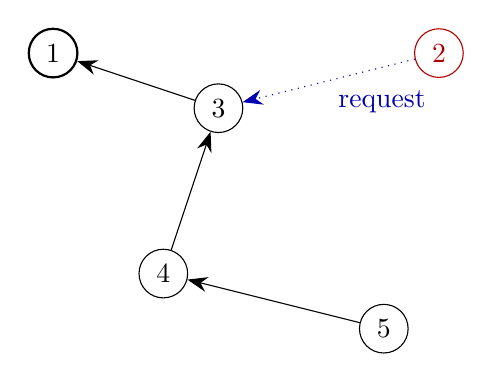
\begin{tikzpicture}
[bn/.style={circle,draw}
,root/.style={bn,thick}
,be/.style={draw=black,arrows={-Stealth[scale=1.5]}}
,req/.style={bn,red!70!black}
,auto,scale=0.7]
\node[root] (n1) at (0,5) {1};
\node[req] (n2) at (7,5) {2};
\node[bn] (n3) at (3,4) {3};
\node[bn] (n4) at (2,1) {4};
\node[bn] (n5) at (6,0) {5};
\draw[be] (n4) -- (n3);
\draw[be] (n5) -- (n4);
\draw[be] (n3) -- (n1);
\draw[be,dotted,blue!70!black] (n2) -- node{request} (n3);
\end{tikzpicture}
\caption{Node 2 sends a request towards its parent after which it sets its parent to itself to become a root}
\end{subfigure}

\begin{subfigure}[t]{0.5\textwidth}
\centering
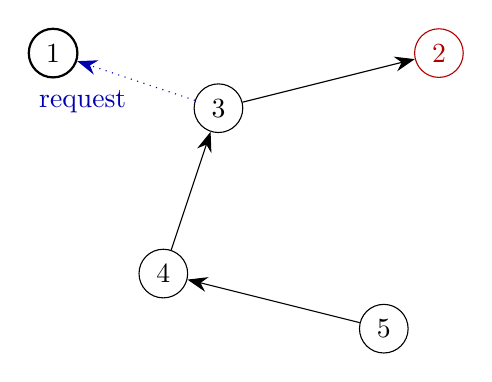
\begin{tikzpicture}
[bn/.style={circle,draw}
,root/.style={bn,thick}
,be/.style={draw=black,arrows={-Stealth[scale=1.5]}}
,req/.style={bn,red!70!black}
,auto,scale=0.7]
\node[root] (n1) at (0,5) {1};
\node[req] (n2) at (7,5) {2};
\node[bn] (n3) at (3,4) {3};
\node[bn] (n4) at (2,1) {4};
\node[bn] (n5) at (6,0) {5};
\draw[be] (n4) -- (n3);
\draw[be] (n5) -- (n4);
\draw[be] (n3) -- (n2);
\draw[be,dotted,blue!70!black] (n3) -- node{request} (n1);
\end{tikzpicture}
\caption{Node 3 receives the request and forwards it to its parent while changing its parent to the node it received the request from}
\end{subfigure}
\quad
\begin{subfigure}[t]{0.5\textwidth}
\centering
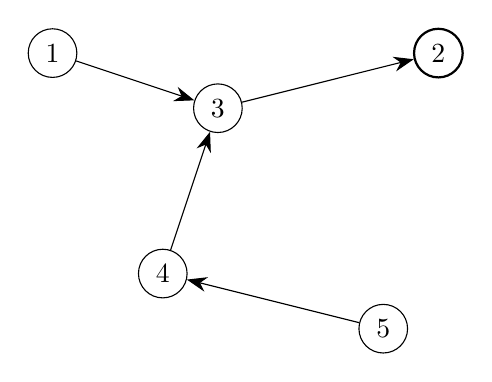
\begin{tikzpicture}
[bn/.style={circle,draw}
,root/.style={bn,thick}
,be/.style={draw=black,arrows={-Stealth[scale=1.5]}}
,req/.style={bn,red!70!black}
,auto,scale=0.7]
\node[bn] (n1) at (0,5) {1};
\node[root] (n2) at (7,5) {2};
\node[bn] (n3) at (3,4) {3};
\node[bn] (n4) at (2,1) {4};
\node[bn] (n5) at (6,0) {5};
\draw[be] (n4) -- (n3);
\draw[be] (n5) -- (n4);
\draw[be] (n3) -- (n2);
\draw[be] (n1) -- (n3);
\end{tikzpicture}
\caption{Node 1 which has the token receives the request, it sends the token to 2, making it the new root. It sets its parent to the node it received the request from}
\end{subfigure}

\begin{subfigure}[t]{0.5\textwidth}
\centering
\begin{tikzpicture}
[bn/.style={circle,draw}
,root/.style={bn,thick}
,be/.style={draw=black,arrows={-Stealth[scale=1.5]}}
,req/.style={bn,red!70!black}
,auto,scale=0.7]
\node[bn] (n1) at (0,5) {1};
\node[root] (n2) at (7,5) {2};
\node[bn] (n3) at (3,4) {3};
\node[bn] (n4) at (2,1) {4};
\node[req] (n5) at (6,0) {5};
\node[above=0 of n5, red!70!black] {needs token};
\draw[be] (n4) -- (n3);
\draw[be] (n5) -- (n4);
\draw[be] (n3) -- (n2);
\draw[be] (n1) -- (n3);
\draw[be,dotted,blue!70!black] (n5) .. controls (n4) and (n3) .. node[right]{request} (n2);
\end{tikzpicture}
\caption{Node 5 needs the token, resulting in a request path over $\{5,4,3,2\}$}
\end{subfigure}
\quad
\begin{subfigure}[t]{0.5\textwidth}
\centering
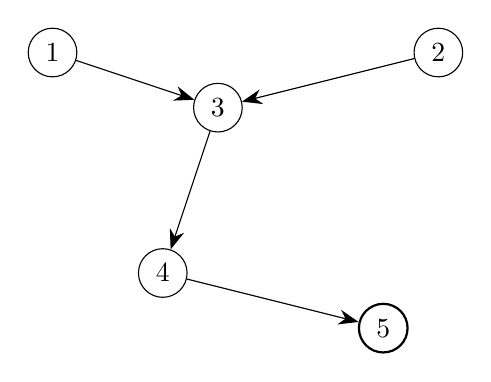
\begin{tikzpicture}
[bn/.style={circle,draw}
,root/.style={bn,thick}
,be/.style={draw=black,arrows={-Stealth[scale=1.5]}}
,req/.style={bn,red!70!black}
,auto,scale=0.7]
\node[bn] (n1) at (0,5) {1};
\node[bn] (n2) at (7,5) {2};
\node[bn] (n3) at (3,4) {3};
\node[bn] (n4) at (2,1) {4};
\node[root] (n5) at (6,0) {5};
\draw[be] (n2) -- (n3);
\draw[be] (n4) -- (n5);
\draw[be] (n3) -- (n4);
\draw[be] (n1) -- (n3);
\end{tikzpicture}
\caption{After node 2 with the token received the request it sent it to node 5. The nodes 4, 3 and 2 on the request path inverted the direction of their arrows}
\end{subfigure}
\caption{Arrow example}
\label{fig:arrow}
\end{figure}

\TODO{Abstract drawing stuff, perhaps implement Arvy in \LaTeX?}

\subsection{Ivy}
\label{intro:ivy}

Ivy encompasses an entirely different way to invert the arrows along the request path, namely that every node $a^{(i+1)}$ receiving the request sets its parent to the node that made the original request: $parent(a^{(i+1)})=a^{(0)}$. Therefore $a^{(0)}$ ends up being the center of a star consisting of all nodes along the request path. Figure~\ref{fig:ivy} shows an example of Ivy.

Ivy was originally described in \cite{Ivy}.

\begin{figure}[]
\begin{subfigure}[t]{0.5\textwidth}
\centering
\begin{tikzpicture}
[bn/.style={circle,draw}
,root/.style={bn,thick}
,be/.style={draw=black,arrows={-Stealth[scale=1.5]}}
,req/.style={bn,red!70!black}
,auto,scale=0.7]
\node[root] (n1) at (0,5) {1};
\node[req] (n2) at (7,5) {2};
\node[above=0 of n2, red!70!black] {needs token};
\node[bn] (n3) at (3,4) {3};
\node[bn] (n4) at (2,1) {4};
\node[bn] (n5) at (6,0) {5};
\draw[be] (n2) -- (n3);
\draw[be] (n4) -- (n3);
\draw[be] (n5) -- (n4);
\draw[be] (n3) -- (n1);
\end{tikzpicture}
\caption{Node 2 needs the token}
\end{subfigure}
\quad
\begin{subfigure}[t]{0.5\textwidth}
\centering
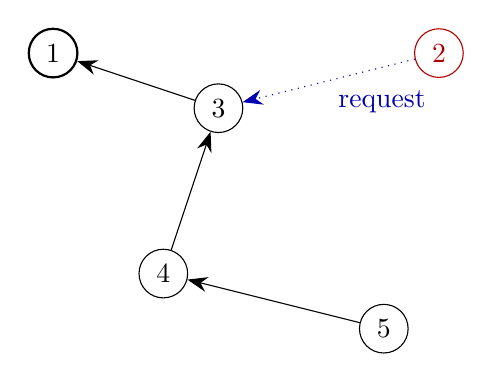
\begin{tikzpicture}
[bn/.style={circle,draw}
,root/.style={bn,thick}
,be/.style={draw=black,arrows={-Stealth[scale=1.5]}}
,req/.style={bn,red!70!black}
,auto,scale=0.7]
\node[root] (n1) at (0,5) {1};
\node[req] (n2) at (7,5) {2};
\node[bn] (n3) at (3,4) {3};
\node[bn] (n4) at (2,1) {4};
\node[bn] (n5) at (6,0) {5};
\draw[be] (n4) -- (n3);
\draw[be] (n5) -- (n4);
\draw[be] (n3) -- (n1);
\draw[be,dotted,blue!70!black] (n2) -- node{request} (n3);
\end{tikzpicture}
\caption{Node 2 sends a request towards its parent after which it sets its parent to itself to become a root}
\end{subfigure}

\begin{subfigure}[t]{0.5\textwidth}
\centering
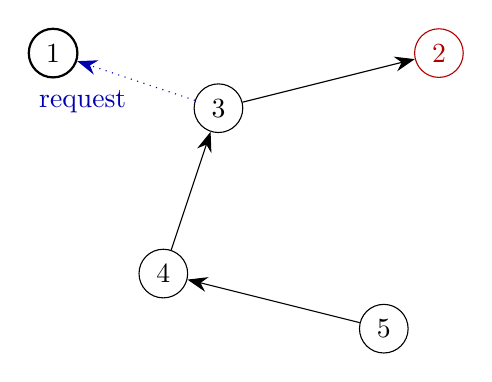
\begin{tikzpicture}
[bn/.style={circle,draw}
,root/.style={bn,thick}
,be/.style={draw=black,arrows={-Stealth[scale=1.5]}}
,req/.style={bn,red!70!black}
,auto,scale=0.7]
\node[root] (n1) at (0,5) {1};
\node[req] (n2) at (7,5) {2};
\node[bn] (n3) at (3,4) {3};
\node[bn] (n4) at (2,1) {4};
\node[bn] (n5) at (6,0) {5};
\draw[be] (n4) -- (n3);
\draw[be] (n5) -- (n4);
\draw[be] (n3) -- (n2);
\draw[be,dotted,blue!70!black] (n3) -- node{request} (n1);
\end{tikzpicture}
\caption{Node 3 receives the request and forwards it to its parent while changing its parent to the node that sent out the initial request}
\end{subfigure}
\quad
\begin{subfigure}[t]{0.5\textwidth}
\centering
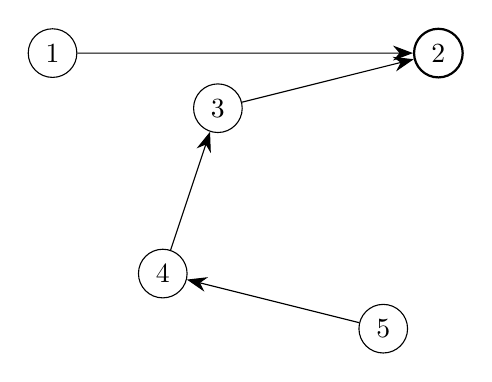
\begin{tikzpicture}
[bn/.style={circle,draw}
,root/.style={bn,thick}
,be/.style={draw=black,arrows={-Stealth[scale=1.5]}}
,req/.style={bn,red!70!black}
,auto,scale=0.7]
\node[bn] (n1) at (0,5) {1};
\node[root] (n2) at (7,5) {2};
\node[bn] (n3) at (3,4) {3};
\node[bn] (n4) at (2,1) {4};
\node[bn] (n5) at (6,0) {5};
\draw[be] (n4) -- (n3);
\draw[be] (n5) -- (n4);
\draw[be] (n3) -- (n2);
\draw[be] (n1) -- (n2);
\end{tikzpicture}
\caption{Node 1 which has the token receives the request, it sends the token to 2, making it the new root. It sets its parent to the node that sent out the initial request as well}
\end{subfigure}

\begin{subfigure}[t]{0.5\textwidth}
\centering
\begin{tikzpicture}
[bn/.style={circle,draw}
,root/.style={bn,thick}
,be/.style={draw=black,arrows={-Stealth[scale=1.5]}}
,req/.style={bn,red!70!black}
,auto,scale=0.7]
\node[bn] (n1) at (0,5) {1};
\node[root] (n2) at (7,5) {2};
\node[bn] (n3) at (3,4) {3};
\node[bn] (n4) at (2,1) {4};
\node[req] (n5) at (6,0) {5};
\node[above=0 of n5, red!70!black] {needs token};
\draw[be] (n4) -- (n3);
\draw[be] (n5) -- (n4);
\draw[be] (n3) -- (n2);
\draw[be] (n1) -- (n2);
\draw[be,dotted,blue!70!black] (n5) .. controls (n4) and (n3) .. node[right]{request} (n2);
\end{tikzpicture}
\caption{Node 5 needs the token, resulting in a request path over $\{5,4,3,2\}$}
\end{subfigure}
\quad
\begin{subfigure}[t]{0.5\textwidth}
\centering
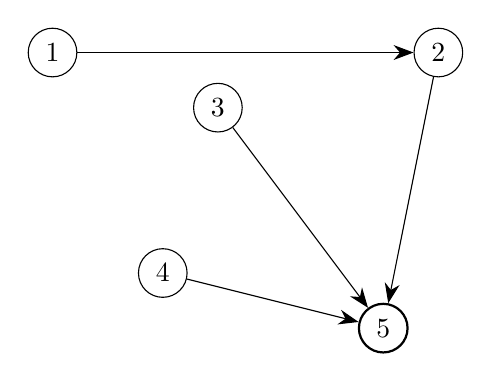
\begin{tikzpicture}
[bn/.style={circle,draw}
,root/.style={bn,thick}
,be/.style={draw=black,arrows={-Stealth[scale=1.5]}}
,req/.style={bn,red!70!black}
,auto,scale=0.7]
\node[bn] (n1) at (0,5) {1};
\node[bn] (n2) at (7,5) {2};
\node[bn] (n3) at (3,4) {3};
\node[bn] (n4) at (2,1) {4};
\node[root] (n5) at (6,0) {5};
\draw[be] (n2) -- (n5);
\draw[be] (n4) -- (n5);
\draw[be] (n3) -- (n5);
\draw[be] (n1) -- (n2);
\end{tikzpicture}
\caption{After node 2 with the token received the request it sent it to node 5. The nodes 4, 3 and 2 on the request path all set their parent to the node that sent out the initial request}
\end{subfigure}
\caption{Ivy example}
\label{fig:ivy}
\end{figure}

\subsection{Arvy}

Arvy generalizes the ideas of Arrow and Ivy by allowing nodes $a^{(i+1)}$ that received a request to set their parent to any node the request already traveled through, so $parent(a^{(i+1)})\in\{a^{(0)},\dots,a^{(i)}\}$. See Figure~\ref{fig:arvy} for an example.

It's easy to see that this algorithm maintains a spanning tree over time with sequential requests and that it's correct. However this also holds for concurrent requests as the paper introducing Arvy~\cite{Arvy} shows.

\begin{figure}[]
\begin{subfigure}[t]{0.5\textwidth}
\centering
\begin{tikzpicture}
[bn/.style={circle,draw}
,root/.style={bn,thick}
,be/.style={draw=black,arrows={-Stealth[scale=1.5]}}
,req/.style={bn,red!70!black}
,auto,scale=0.7]
\node[root] (n1) at (0,5) {1};
\node[req] (n2) at (7,5) {2};
\node[above=0 of n2, red!70!black] {needs token};
\node[bn] (n3) at (3,4) {3};
\node[bn] (n4) at (2,1) {4};
\node[bn] (n5) at (6,0) {5};
\draw[be] (n2) -- (n3);
\draw[be] (n4) -- (n3);
\draw[be] (n5) -- (n4);
\draw[be] (n3) -- (n1);
\end{tikzpicture}
\caption{Node 2 needs the token}
\end{subfigure}
\quad
\begin{subfigure}[t]{0.5\textwidth}
\centering
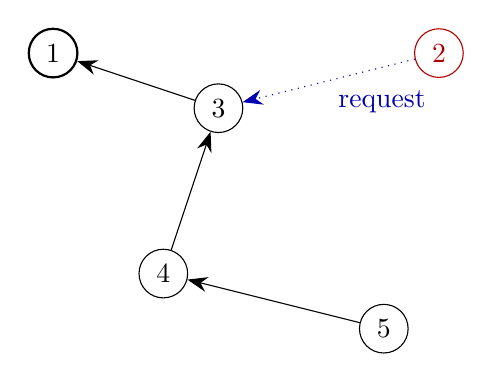
\begin{tikzpicture}
[bn/.style={circle,draw}
,root/.style={bn,thick}
,be/.style={draw=black,arrows={-Stealth[scale=1.5]}}
,req/.style={bn,red!70!black}
,auto,scale=0.7]
\node[root] (n1) at (0,5) {1};
\node[req] (n2) at (7,5) {2};
\node[bn] (n3) at (3,4) {3};
\node[bn] (n4) at (2,1) {4};
\node[bn] (n5) at (6,0) {5};
\draw[be] (n4) -- (n3);
\draw[be] (n5) -- (n4);
\draw[be] (n3) -- (n1);
\draw[be,dotted,blue!70!black] (n2) -- node{request} (n3);
\end{tikzpicture}
\caption{Node 2 sends a request towards its parent after which it sets its parent to itself}
\end{subfigure}

\begin{subfigure}[t]{0.5\textwidth}
\centering
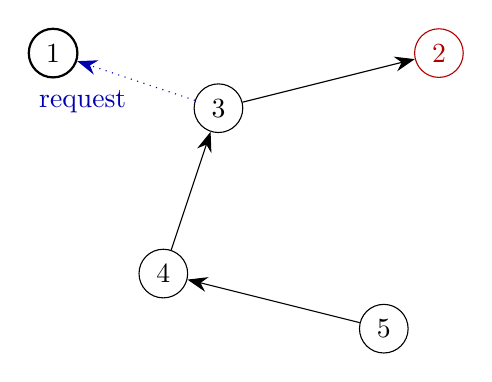
\begin{tikzpicture}
[bn/.style={circle,draw}
,root/.style={bn,thick}
,be/.style={draw=black,arrows={-Stealth[scale=1.5]}}
,req/.style={bn,red!70!black}
,auto,scale=0.7]
\node[root] (n1) at (0,5) {1};
\node[req] (n2) at (7,5) {2};
\node[bn] (n3) at (3,4) {3};
\node[bn] (n4) at (2,1) {4};
\node[bn] (n5) at (6,0) {5};
\draw[be] (n4) -- (n3);
\draw[be] (n5) -- (n4);
\draw[be] (n3) -- (n2);
\draw[be,dotted,blue!70!black] (n3) -- node{request} (n1);
\end{tikzpicture}
\caption{Node 3 receives the request and forwards it to its parent while changing its parent to the only previously visited node 2}
\end{subfigure}
\quad
\begin{subfigure}[t]{0.5\textwidth}
\centering
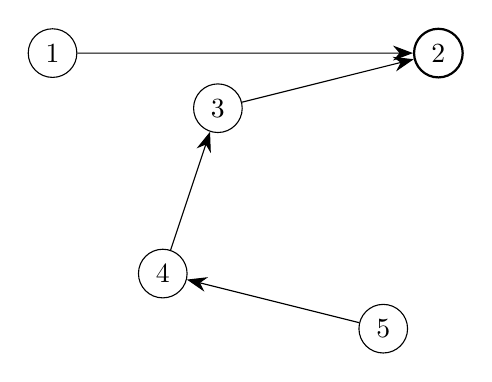
\begin{tikzpicture}
[bn/.style={circle,draw}
,root/.style={bn,thick}
,be/.style={draw=black,arrows={-Stealth[scale=1.5]}}
,req/.style={bn,red!70!black}
,auto,scale=0.7]
\node[bn] (n1) at (0,5) {1};
\node[root] (n2) at (7,5) {2};
\node[bn] (n3) at (3,4) {3};
\node[bn] (n4) at (2,1) {4};
\node[bn] (n5) at (6,0) {5};
\draw[be] (n4) -- (n3);
\draw[be] (n5) -- (n4);
\draw[be] (n3) -- (n2);
\draw[be] (n1) -- (n2);
\end{tikzpicture}
\caption{Node 1 which has the token receives the request, it sends the token to 2, making it the new root. Out of the possible new parents $\{2,3\}$ it chooses 2}
\end{subfigure}

\begin{subfigure}[t]{0.5\textwidth}
\centering
\begin{tikzpicture}
[bn/.style={circle,draw}
,root/.style={bn,thick}
,be/.style={draw=black,arrows={-Stealth[scale=1.5]}}
,req/.style={bn,red!70!black}
,auto,scale=0.7]
\node[bn] (n1) at (0,5) {1};
\node[root] (n2) at (7,5) {2};
\node[bn] (n3) at (3,4) {3};
\node[bn] (n4) at (2,1) {4};
\node[req] (n5) at (6,0) {5};
\node[above=0 of n5, red!70!black] {needs token};
\draw[be] (n4) -- (n3);
\draw[be] (n5) -- (n4);
\draw[be] (n3) -- (n2);
\draw[be] (n1) -- (n2);
\draw[be,dotted,blue!70!black] (n5) .. controls (n4) and (n3) .. node[right]{request} (n2);
\end{tikzpicture}
\caption{Node 5 needs the token, resulting in a request path over $\{5,4,3,2\}$}
\end{subfigure}
\quad
\begin{subfigure}[t]{0.5\textwidth}
\centering
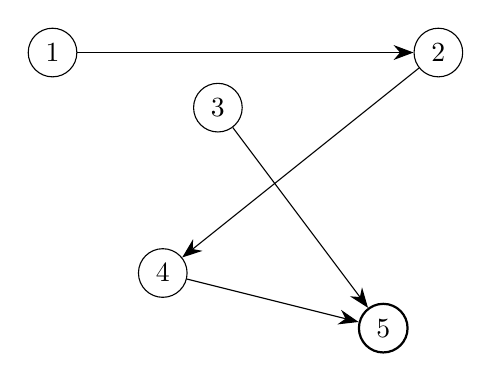
\begin{tikzpicture}
[bn/.style={circle,draw}
,root/.style={bn,thick}
,be/.style={draw=black,arrows={-Stealth[scale=1.5]}}
,req/.style={bn,red!70!black}
,auto,scale=0.7]
\node[bn] (n1) at (0,5) {1};
\node[bn] (n2) at (7,5) {2};
\node[bn] (n3) at (3,4) {3};
\node[bn] (n4) at (2,1) {4};
\node[root] (n5) at (6,0) {5};
\draw[be] (n2) -- (n4);
\draw[be] (n4) -- (n5);
\draw[be] (n3) -- (n5);
\draw[be] (n1) -- (n2);
\end{tikzpicture}
\caption{After node 2 with the token received the request it sent it to node 5. The nodes 4, 3 and 2 on the request path were able to choose its new parent from $\{5\}$, $\{5,4\}$ and $\{5,4,3\}$ respectively.}
\end{subfigure}
\caption{Arvy example}
\label{fig:arvy}
\end{figure}


\chapter{Algorithms}

This section describes all the Arvy algorithms to be tested. A simplified version of a general algorithm can be written as follows, which we'll be using in the following sections. Note that the request path is denoted as $\{a_i\}$ as in previous sections.

\begin{algorithm}
\caption{Arvy algorithm}
\label{arvyalg}
\begin{algorithmic}
\Function{RequestToken}{$a_0$}
\Comment Node $a_0$ wants the token
\If{$parent(a_0)\neq a_0$}
    \State send request for token to $parent(a_0)$
    \State $parent(a_0)\gets a_0$
\EndIf
\EndFunction
\Function{ReceiveRequest}{$a_k$}
\Comment Node $a_k$ receives a request for the token
\If{$parent(a_k)=a_k$}
    \State send token to $a_0$
\Else
    \State forward request to $parent(a_k)$
\EndIf
\State $parent(a_k)\gets\;$\Call{SelectNewParent}{$a_0, a_1, \dots, a_{k-1}$}
\EndFunction
\Function{SelectNewParent}{$\{a_0, a_1,\dots,a_{k-1}\}$}
\Comment Selects a new parent to connect to
\State\Return any of $a_i$
\EndFunction
\end{algorithmic}
\end{algorithm}

Any concrete algorithm will have to define an implementation of $\textsc{SelectNewParent}$. 

\section{Arrow}

As already explained in section~\ref{intro:arrow}, Arrow maintains the structure of the spanning tree by always selecting the most recent node as a new parent, therefore inverting the arrows.
\begin{algorithmic}
\Function{SelectNewParent}{$\{a_0, a_1,\dots,a_{k-1}\}$}
\State\Return $a_{k-1}$
\EndFunction
\end{algorithmic}

\section{Ivy}

Also explained already in section~\ref{intro:ivy}, Ivy always connects every node along a request path to the node that made the original request.
\begin{algorithmic}
\Function{SelectNewParent}{$\{a_0, a_1,\dots,a_{k-1}\}$}
\State\Return $a_0$
\EndFunction
\end{algorithmic}

\section{Edge Cost Minimizer}

Since algorithms have access to the edge costs, we should make use of those. One simple first algorithm one can think of is one that always chooses the node with minimum edge cost as the new parent. See figure~\ref{fig:ecm} for an example. This heuristic intuitively should perform well since short paths make for short request paths.
\begin{algorithmic}
\Function{SelectNewParent}{$\{a_0, a_1,\dots,a_{k-1}\}$}
\State\Return$a_i$ such that $c(a_k,a_i),i\in\{0,\dots,k-1\}$ is minimal
\EndFunction
\end{algorithmic}

Notable properties of this algorithm include
\begin{itemize}
\item The total edge distance in the tree can only get smaller over time, since a previous edge between $a_{k-1}$ and $a_k$ can only be replaced with a shorter one, which will be the same edge when $c(a_k,a_{k-1})$ is the minimum already.
\item This in turn means that with a good enough distribution of nodes initiating requests, the tree will converge to a Minimum Spanning Tree (MST) eventually, because that's the state of lowest possible total edge distance.
\item Consequently, once the tree has converged, this algorithm behaves exactly the same as Arrow, which never changes the tree by design. Therefore to get the eventual behavior of this algorithm, one can simply start with an MST directly and run Arrow. This seems to imply that in general this Algorithm isn't any more powerful than Arrow.
\end{itemize}

\begin{figure}
\begin{subfigure}[t]{0.5\textwidth}
\centering
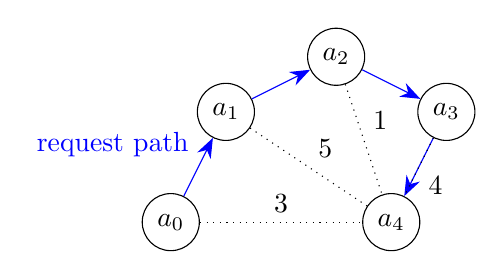
\begin{tikzpicture}
[bn/.style={circle,draw}
,root/.style={bn,thick}
,be/.style={draw=blue,arrows={-Stealth[scale=1.5]}}
,req/.style={bn,red!70!black}
,auto,scale=0.7]
\node[bn] (n1) at (0,0) {$a_0$};
\node[bn] (n2) at (1,2) {$a_1$};
\node[bn] (n3) at (3,3) {$a_2$};
\node[bn] (n4) at (5,2) {$a_3$};
\node[bn] (n5) at (4,0) {$a_4$};
\draw[be] (n1) -- node[blue]{request path} (n2);
\draw[be] (n2) -- (n3);
\draw[be] (n3) -- (n4);
\draw[be] (n4) -- (n5);
\draw[dotted] (n1) -- node{$3$} (n5);
\draw[dotted] (n2) -- node{$5$} (n5);
\draw[dotted] (n3) -- node{$1$} (n5);
\draw[dotted] (n4) -- node{$4$} (n5);
\end{tikzpicture}
\caption{The request arrives at $a_4$ which now needs to decide which one of $a_0,\dots a_3$ to choose as a parent. For this it can access the edge costs to all of them.}
\end{subfigure}
\quad
\begin{subfigure}[t]{0.5\textwidth}
\centering
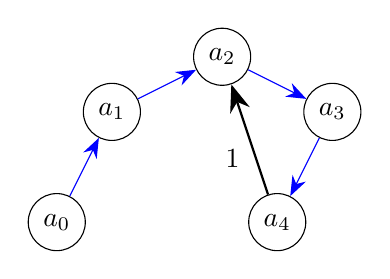
\begin{tikzpicture}
[bn/.style={circle,draw}
,root/.style={bn,thick}
,be/.style={draw=blue,arrows={-Stealth[scale=1.5]}}
,req/.style={bn,red!70!black}
,auto,scale=0.7]
\node[bn] (n1) at (0,0) {$a_0$};
\node[bn] (n2) at (1,2) {$a_1$};
\node[bn] (n3) at (3,3) {$a_2$};
\node[bn] (n4) at (5,2) {$a_3$};
\node[bn] (n5) at (4,0) {$a_4$};
\draw[be] (n1) -- (n2);
\draw[be] (n2) -- (n3);
\draw[be] (n3) -- (n4);
\draw[be] (n4) -- (n5);
\draw[thick,arrows={-Stealth[scale=1.5]}] (n5) -- node{$1$} (n3);
\end{tikzpicture}
\caption{$a_2$ gets chosen as the new parent since the edge towards it has the smallest cost.}
\end{subfigure}
\caption{Edge Cost Minimizer example with a fourth node in the request path.}
\label{fig:ecm}
\end{figure}

\section{Fixed Path Ratio}

Another simple algorithm we'll call Fixed Path Ratio (FPR), which chooses the node at a fixed ratio $f\in[0,1]$ between the first and the last one. As an example, with a request path $a_0,a_1,a_2,a_3,a_4$ and a fixed ratio of $f=\frac{1}{2}$, node $a_5$ would choose $a_2$ as its new parent, since it's half-way between $a_0$ and $a_4$. We use the earlier node in case of a ratio being inbetween two nodes. See figure~\ref{fig:fpr} for an example.

\begin{algorithmic}
\Function{SelectNewParent}{$\{a_0, a_1,\dots,a_{k-1}\}$}
\State\Return $a_{\lfloor f(k-1)\rfloor}$
\EndFunction
\end{algorithmic}

A variation of this algorithm FPR' doesn't use the fraction on the node counts, but on the edge costs instead. A request path $a_0,a_1,a_2,\dots,a_{k-1}$ gets mapped to costs $c'_i$ representing how far the request had to travel to get to node $a_i$. These costs are defined as
\begin{equation}
c'_i=\sum_{j=1}^ic(a_{j-1},a_j)
\end{equation}

The last node whose $c'$ is lower than or equal to $f\cdot c'_{k-1}$ is then selected.

\begin{algorithmic}
\Function{SelectNewParent}{$\{a_0, a_1,\dots,a_{k-1}\}$}
\State\Return $a_i$ with the maximum $i$ with the constraint $c'_i\leq f\cdot c'_{k-1}$ 
\EndFunction
\end{algorithmic}

This algorithm has the following interesting properties:
\begin{itemize}
\item For $f=0$ these algorithms are equivalent to Ivy. Similarly $f=1$ is equivalent to Arrow.
\item For $f=\frac{1}{2}$, FPR builds a binary tree on the request path, see figure~\ref{fig:fpr} for an example.
\item With $c(u,v)=const\;\forall u,v$ FPR' is equivalent to FPR.

\end{itemize}

\begin{figure}
\centering
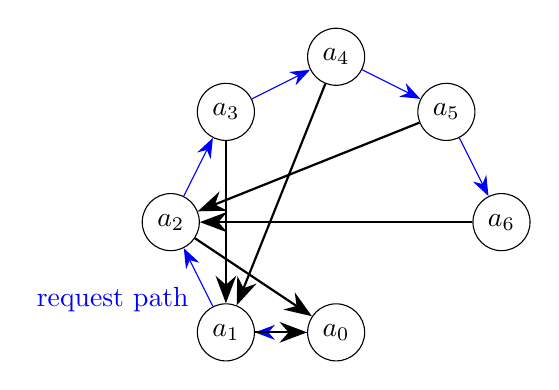
\begin{tikzpicture}
[bn/.style={circle,draw}
,root/.style={bn,thick}
,be/.style={thick,arrows={-Stealth[scale=1.5]}}
,pe/.style={draw=blue,arrows={-Stealth[scale=1.5]}}
,req/.style={bn,red!70!black}
,auto,scale=0.7]
\node[bn] (n0) at (3,0) {$a_0$};
\node[bn] (n1) at (1,0) {$a_1$};
\node[bn] (n2) at (0,2) {$a_2$};
\node[bn] (n3) at (1,4) {$a_3$};
\node[bn] (n4) at (3,5) {$a_4$};
\node[bn] (n5) at (5,4) {$a_5$};
\node[bn] (n6) at (6,2) {$a_6$};

\draw[pe] (n0) -- (n1);
\draw[pe] (n1) -- node[blue]{request path} (n2);
\draw[pe] (n2) -- (n3);
\draw[pe] (n3) -- (n4);
\draw[pe] (n4) -- (n5);
\draw[pe] (n5) -- (n6);

\draw[be] (n1) -- (n0);
\draw[be] (n2) -- (n0);
\draw[be] (n3) -- (n1);
\draw[be] (n4) -- (n1);
\draw[be] (n5) -- (n2);
\draw[be] (n6) -- (n2);
\end{tikzpicture}
\caption{FPR algorithm with a ratio of $\frac{1}{2}$ and a request path of 7 nodes. A binary tree is created.}
\label{fig:fpr}
\end{figure}

\section{Uniformly Random}

Not a particularly interesting algorithm, but good as a reference point is a completely random algorithm, selecting a new parent uniformly random from all available choices.

\begin{algorithmic}
\Function{SelectNewParent}{$\{a_0, a_1,\dots,a_{k-1}\}$}
\State\Return choose $a_i$ uniformly at random
\EndFunction
\end{algorithmic}

\section{Dynamic Star}

As \cite{Peleg} showed, the best shortest path tree is a pretty good tree to use for Arrow if you know the probability distribution $p_i, i\in V$ of nodes making requests. A shortest path tree is a tree with a specific center node, while all others are connected to the center through a shortest path between them \TODO{Explain best shortest path tree}. Since we're dealing with a complete graph and metric costs, the direct edge between two nodes is always a shortest path, which when applied to all nodes results in a star-shaped tree with the center node connected directly to all others.

This Dynamic Star algorithm measures the distribution $p_i$ at runtime and dynamically adjusts the tree according to it, striving for a star. The fact that Arvy is a distributed algorithm however poses a problem, as a node can't obtain a global view of the system to get accurate values for $p_i$, so we'll have to make do with every node $v$ having a local approximation $p_i^v$ of $p_i$.

The idea is that each node $v\in V$ maintains a count $n_i^v\in\mathbb{N}_0$ of how many times node $i\in V$ made a request, initialized with all $0$. Because $v$ always knows how many requests it made itself, the value for $n_v^v$ is indeed accurate, while all others can be an outdated value, meaning $\forall i:n_v^i\leq n_v^v$. $n_i^v$ gets updated according to the following rules:
\begin{enumerate}
\item When node $v$ makes a request, set $n_v^v\gets n_v^v+1$
\label{rule1}
\item Any message sent from $v$ shall include a subset of known counts $\{n_i^v,i\in S\subset V\}$, which when arriving at $u$ will update all received values if they are bigger than the values already known: $n_i^u\gets \max(n_i^u,n_i^v),i\in S$.
\end{enumerate}

Depending on the choice of the subset $S$ of value updates to send, the information propagation of the true values in the network might be slower or faster. Generally the bigger $|S|$, the faster information propagates. Some interesting choices for $S$ are
\begin{itemize}
\item On a request path $\{a_0,a_1,\dots\}$, $a_0$ only sends along its own count $S=\{n_{a_0}^{a_0}\}$, while all nodes along the path forward this $S$. Therefore all $a_i$ will momentarily know the accurate value for $n_{a_0}^{a_i}$.
\item With $S=V$ we get as much information propagation as possible, but also $\mathcal{O}(n)$ message complexity.
\item Message size can be reduced by making $S$ a uniform random selection of $V$, with $|S|\ll|V|$. With many requests happening, information should still propagate rather quickly.
\item An improved version of this is a random weighted selection, preferring $n_i^v$ that have been updated more recently.
\end{itemize}

Once such $n_i^v$ are known, the approximated request probabilities $p_i^v$ are then simply
\begin{equation}
p_i^v=\frac{n_i^v}{\sum_jn_j^v}
\end{equation}

We then define the cost of a star tree with node $k$ in the center as follows:
\begin{equation}
c_{star}^k=\sum_{i,j}p_i^vp_j^v(c(i, k)+c(k,j))
\end{equation}

With this we have everything in place for the algorithm to select a new parent out of the available options $\{a_0,a_1,\dots,a_{k-1}\}$. We do so by selecting the $a_i$ with the lowest cost as the center of the star.

\begin{algorithmic}
\Function{SelectNewParent}{$\{a_0, a_1,\dots,a_{k-1}\}$}
\State\Return Choose $a_i$ with lowest $c_{star}^{a_i}$
\EndFunction
\end{algorithmic}

Justification is needed for the fact that the node $a_k$ selecting the new parent seems to access costs not imminent to it, which was given as a restriction in \ref{model}. This can be circumvented by each node $a_i$ calculating $c_{star}^{a_i}$ locally, then sending that value in the message to $a_{i+1}$. This is however not the same as calculating all $c_{star}$ values in the final node in the request path, but the resulting values shouldn't be far off.

Note that this algorithm needs $\mathcal{O}(n^2)$ time for calculation of $c_{star}$ in each node along the request path, making it very slow to run in comparison to other algorithms. Messages only need to send the $S$ and the $a_i$ with lowest $c_{star}^{a_i}$, making message complexity $\mathcal{O}(|S|)$.

\subsection{Non-converging Dynamic Star}

One slight problem with the Dynamic Star algorithm is that in general it eventually converges to a static tree. This is because as the total number of request grows bigger, changes to $n_i^v$ matter less and less. After $R\in\mathbb{N}$ requests, another request can cause a maximum change to $p_i^v$ of
\begin{equation}
\begin{split}
\left|p_i^v-p_i^{'v}\right| = & \left|\frac{n_i^v}{\sum_jn_j^v}-\frac{n_i^{'v}}{\sum_jn_j^{'v}}\right| = \left|\frac{n_i^v}{R}-\frac{n_i^v+\{0,1\}}{R+1}\right| \\
= & \left|\frac{n_i^vR+n_i^v-n_i^vR+\{0,1\}R}{R(R+1)}\right| = \frac{\left|n_i^v-\{0,1\}R\right|}{R(R+1)} \\
\leq & \frac{R}{R(R+1)}=\frac{1}{R+1}\to_{R\to\infty} 0
\end{split}
\end{equation}

Where $\{0,1\}$ is $1$ or $0$ depending on whether $n_i^v$ was increased or not.

This is a problem because it means the longer a system runs, the less it's adapting to changes in the probability pattern. If after $10^{100}$ requests a request-controlling adversary shows up, it could exploit this practically static tree by constantly bouncing requests between two nodes with the worst connection. If this were to happen initially it wouldn't be a problem as the heuristic could adapt to this by choosing a better star center quickly. This means the algorithm's behavior is dependent on how long it has been running.

The general idea to solve this problem is to give less weight to older requests. This can be done in multiple ways:
\begin{itemize}
\item After every increment of $n_i^v$ by one, all counts get decreased by a constant factor: $\forall i:n_i^v\gets \alpha n_i^v$ with $0<\alpha<1$. If this was a global view this would work well, since after $R$ requests an original contribution to $n_i^{global}$ of $1$ would be reduced to $\alpha^R$, implementing an exponential weight falloff. However since this is not a global view, it won't work as well, because depending on the propagation speed with $|S|$, the $n_i^v$ will be more outdated, resulting in old requests having more weight than they would in a global view.
\item A slight improvement over this can be achieved: For each message sent from $v$, the total amount of requests known $\sum_jn_j^v$ is sent as well. When received by $u$, it's possible for it to calculate the difference of known requests $dR=\sum_jn_j^v-\sum_jn_j^u$. This means all $n_i^u$ are about that many requests more in the past than $n_i^v$, so an update is done on them to compensate for this: $\forall i:n_i^u\gets\alpha^{dR}n_i^u$. This is better because the multiplication with $\alpha$ doesn't depend on the selection of $|S|$ anymore, resulting in older values being more accurately weighed.
\item With the requirement of nodes being able to measure passing of time, it's possible to improve on this: Every $dt$ time units, all counts get decreased with the constant factor $\forall i:n_i^v\gets \alpha n_i^v$. This is now a accurate time-based exponential falloff, which is independent of both the propagation speed and the request pattern.
\end{itemize}

In this thesis we assume that the request pattern is periodic, where this is not a big problem. Therefore this Non-converging Dynamic Star algorithm is not further evaluated.

\section{Recursive Clique}

As we'll see in section~\ref{result:clique}, Ivy performs well on cliques of less than 5 nodes. Taking advantage of this fact, we design a graph resembling a clique, but where each node can contain another clique within, and so on. See figure~\ref{fig:reclique} for an example with 2 layers of cliques and each layer having a clique of 3 nodes. This resulting recursive clique graph allows running Ivy recursively, taking advantage of Ivy's performance in each recursion level.

A recursive clique graph has a level count parameter $l$ representing the number of levels and a base parameter $b$ for the number of nodes in a clique on a single level. We call the $b$ nodes in all layers except the lowest one \textit{virtual}, because they only exist to group non-virtual nodes in lower layers together. The total number of nodes in such a graph is $b^l$. In addition, for defining costs between edges, we declare a parameter $f>1$ for the increase factor in edge distance between one level. This factor represents how far apart nodes in higher levels are. We define nodes in a clique in the lowest level to have distance $1$ from each other. For arbitrary nodes we can define the cost as

\begin{equation}
c(u,v)=\begin{cases}
0 & \text{if $u=v$} \\
1 & \text{otherwise if $u$ and $v$ share the same lowest layer} \\
f & \text{otherwise if $u$ and $v$ share the same second-lowest layer} \\
f^2 & \text{otherwise if $u$ and $v$ share the same third-lowest layer} \\
\vdots & \\
f^{l-1} & \text{otherwise, $u$ and $v$ are in different nodes of the highest layer} \\
\end{cases}
\end{equation}

When running a recursive Ivy algorithm on such a graph, the guiding rules are:
\begin{enumerate}
\item The spanning tree can only include at most one connection between all virtual nodes on a single layer. This ensures that if a request was made from within the virtual node where the token currently is at, the request path does not exit that virtual node. In addition this means there a request path can include at most $b-1$ edges of length $f^{l-1}$ from the most upper layer (and similarly for lower layers), therefore keeping the number of long edges at a minimum.
\label{reclique-rule-conn}
\item Connect to the earliest possible node in the request path. This ensures that the inverted arrows on the request path lead future requests to the root on the fastest way possible while still satisfying rule \ref{reclique-rule-conn}. This gives Ivy-like behavior on each layer and across layers.
\label{reclique-rule-early}
\end{enumerate}

See figure~\ref{fig:reclique-alg} for an example of how this algorithm behaves.

While in this algorithm we only limit ourselves to these three parameters for simplicity, this idea can be extended much further: Each layer can contain arbitrary graphs without regularity. As an example, with three nodes at the top-most layer, the first node could contain a subgraph of a star, the second node a ring graph and the third node another graph containing more subgraphs for each node. This then also calls for running different Arvy algorithms on each layer, using whichever works best for that layers graph. This is therefore very flexible. In a realistic scenario, the top-most layer can represent different data centers around the world, the layer below different racks in the data center and the layer below that different machines in a rack.

\begin{figure}
\centering
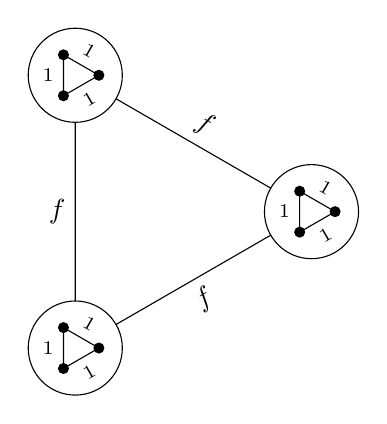
\begin{tikzpicture}
\coordinate (A) at (0:2);
\path (A) +(0:0.3) coordinate (AA);
\path (A) +(120:0.3) coordinate (AB);
\path (A) +(240:0.3) coordinate (AC);
\coordinate (B) at (120:2);
\path (B) +(0:0.3) coordinate (BA);
\path (B) +(120:0.3) coordinate (BB);
\path (B) +(240:0.3) coordinate (BC);
\coordinate (C) at (240:2);
\path (C) +(0:0.3) coordinate (CA);
\path (C) +(120:0.3) coordinate (CB);
\path (C) +(240:0.3) coordinate (CC);

\draw (A) -- node[above,sloped]{$f$} (B) -- node[left]{$f$} (C) -- node[below,sloped]{$f$} (A);

\fill[white] (A) circle [radius=17pt];
\fill[white] (B) circle [radius=17pt];
\fill[white] (C) circle [radius=17pt];
\draw (A) circle [radius=17pt];
\draw (B) circle [radius=17pt];
\draw (C) circle [radius=17pt];

\foreach \x in {A,B,C}
  \foreach \y in {A,B,C}
    \fill (\x\y) circle [radius=2pt];

\draw (AA) -- node[above,sloped]{\scriptsize{1}} (AB) -- node[left]{\scriptsize{1}} (AC) -- node[below,sloped]{\scriptsize{1}} (AA);
\draw (BA) -- node[above,sloped]{\scriptsize{1}} (BB) -- node[left]{\scriptsize{1}} (BC) -- node[below,sloped]{\scriptsize{1}} (BA);
\draw (CA) -- node[above,sloped]{\scriptsize{1}} (CB) -- node[left]{\scriptsize{1}} (CC) -- node[below,sloped]{\scriptsize{1}} (CA);

\end{tikzpicture}
\caption{Recursive Clique graph with 2 levels and 3 nodes in each level. Nodes in the same lowest layer clique have distance $1$ between them, while nodes in different lowest layer cliques have distance $f$ between them.}
\label{fig:reclique}
\end{figure}


\begin{figure}
\begin{subfigure}[t]{0.5\textwidth}
\centering
\begin{tikzpicture}
[be/.style={draw=black,arrows={-Stealth[scale=1.5]}}]
\coordinate (A) at (0:1.8);
\path (A) +(0:0.5) coordinate (AA);
\path (A) +(120:0.5) coordinate (AB);
\path (A) +(240:0.5) coordinate (AC);
\coordinate (B) at (120:1.8);
\path (B) +(0:0.5) coordinate (BA);
\path (B) +(120:0.5) coordinate (BB);
\path (B) +(240:0.5) coordinate (BC);
\coordinate (C) at (240:1.8);
\path (C) +(0:0.5) coordinate (CA);
\path (C) +(120:0.5) coordinate (CB);
\path (C) +(240:0.5) coordinate (CC);

\draw[be] (AB) -- (AA);
\draw[be] (AC) -- (AA);
\draw[be] (BB) -- (BA);
\draw[be] (BC) -- (BA);
\draw[be] (CB) -- (CA);
\draw[be] (CC) -- (CA);
\draw[be] (BA) to[out=0,in=90] (AA);
\draw[be] (CA) to[out=0,in=-90] (AA);

\foreach \x in {A,B,C}
  \foreach \y in {A,B,C}
    \fill (\x\y) circle [radius=2pt];

\fill[red] (CC) circle [radius=2pt,fill=red];
\node[below=0 of CC] {\scriptsize{$a_0$}};
\node[below right=0 and -5pt of CA] {\scriptsize{$a_1$}};
\node[right=0 of AA] {\scriptsize{$a_2$}};

\end{tikzpicture}
\caption{The first node $a_0$ on the request path makes a request for the token which lies at root node $a_2$. $a_2$ will invert its arrow to point to $a_0$ with a long edge, which rule~\ref{reclique-rule-conn} allows because the previous long edge $(a_1,a_2)$ is discarded when the request traverses it.}
\label{fig:reclique-alg-a}
\end{subfigure}
\quad
\begin{subfigure}[t]{0.5\textwidth}
\centering
\begin{tikzpicture}
[be/.style={draw=black,arrows={-Stealth[scale=1.5]}}]
\coordinate (A) at (0:1.8);
\path (A) +(0:0.5) coordinate (AA);
\path (A) +(120:0.5) coordinate (AB);
\path (A) +(240:0.5) coordinate (AC);
\coordinate (B) at (120:1.8);
\path (B) +(0:0.5) coordinate (BA);
\path (B) +(120:0.5) coordinate (BB);
\path (B) +(240:0.5) coordinate (BC);
\coordinate (C) at (240:1.8);
\path (C) +(0:0.5) coordinate (CA);
\path (C) +(120:0.5) coordinate (CB);
\path (C) +(240:0.5) coordinate (CC);

\draw[be] (AB) -- (AA);
\draw[be] (AC) -- (AA);
\draw[be] (BB) -- (BA);
\draw[be] (BC) -- (BA);
\draw[be] (CB) -- (CA);
\draw[be] (CA) -- (CC);
\draw[be] (BA) to[out=0,in=90] (AA);
\draw[be] (AA) to[out=-90,in=-20] (CC);

\foreach \x in {A,B,C}
  \foreach \y in {A,B,C}
    \fill (\x\y) circle [radius=2pt];

\fill[red] (CB) circle [radius=2pt,fill=red];
\node[above=0 of CB] {\scriptsize{$a_0$}};
\node[right=0 of CA] {\scriptsize{$a_1$}};
\node[left=0 of CC] {\scriptsize{$a_2$}};

\end{tikzpicture}
\caption{In the new tree, $a_0$ makes a request for the token at $a_2$ in the same virtual node. As with normal Ivy, all nodes will connect back to the node $a_0$ who made the original request.}
\end{subfigure}

\begin{subfigure}[t]{0.5\textwidth}
\centering
\begin{tikzpicture}
[be/.style={draw=black,arrows={-Stealth[scale=1.5]}}]
\coordinate (A) at (0:1.8);
\path (A) +(0:0.5) coordinate (AA);
\path (A) +(120:0.5) coordinate (AB);
\path (A) +(240:0.5) coordinate (AC);
\coordinate (B) at (120:1.8);
\path (B) +(0:0.5) coordinate (BA);
\path (B) +(120:0.5) coordinate (BB);
\path (B) +(240:0.5) coordinate (BC);
\coordinate (C) at (240:1.8);
\path (C) +(0:0.5) coordinate (CA);
\path (C) +(120:0.5) coordinate (CB);
\path (C) +(240:0.5) coordinate (CC);

\draw[be] (AB) -- (AA);
\draw[be] (AC) -- (AA);
\draw[be] (BB) -- (BA);
\draw[be] (BC) -- (BA);
\draw[be] (CA) -- (CB);
\draw[be] (CC) -- (CB);
\draw[be] (BA) to[out=0,in=90] (AA);
\draw[be] (AA) to[out=-90,in=-20] (CC);

\foreach \x in {A,B,C}
  \foreach \y in {A,B,C}
    \fill (\x\y) circle [radius=2pt];

\fill[red] (BB) circle [radius=2pt,fill=red];
\node[above=0 of BB] {\scriptsize{$a_0$}};
\node[above right=0 and -3pt of BA] {\scriptsize{$a_1$}};
\node[right=0 of AA] {\scriptsize{$a_2$}};
\node[below left=0 and -3pt of CC] {\scriptsize{$a_3$}};
\node[above=0 of CB] {\scriptsize{$a_4$}};

\end{tikzpicture}
\caption{The request path has two long edges, invoking the Ivy behavior on the upper layer: $a_3$ will connect back to $a_0$. Then when $a_4$ receives the request, the rules disallow it from connecting back to $a_0$ as well, since this would lead to multiple edges between virtual nodes. Therefore $a_4$ has to connect back to $a_2$}
\end{subfigure}
\quad
\begin{subfigure}[t]{0.5\textwidth}
\centering
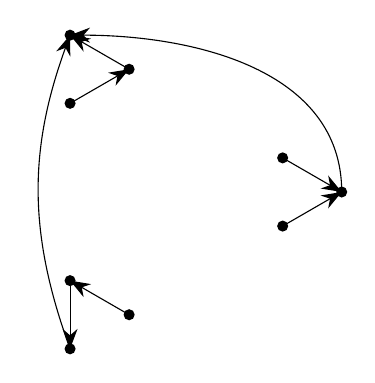
\begin{tikzpicture}
[be/.style={draw=black,arrows={-Stealth[scale=1.5]}}]
\coordinate (A) at (0:1.8);
\path (A) +(0:0.5) coordinate (AA);
\path (A) +(120:0.5) coordinate (AB);
\path (A) +(240:0.5) coordinate (AC);
\coordinate (B) at (120:1.8);
\path (B) +(0:0.5) coordinate (BA);
\path (B) +(120:0.5) coordinate (BB);
\path (B) +(240:0.5) coordinate (BC);
\coordinate (C) at (240:1.8);
\path (C) +(0:0.5) coordinate (CA);
\path (C) +(120:0.5) coordinate (CB);
\path (C) +(240:0.5) coordinate (CC);

\draw[be] (AB) -- (AA);
\draw[be] (AC) -- (AA);
\draw[be] (BA) -- (BB);
\draw[be] (BC) -- (BA);
\draw[be] (CA) -- (CB);
\draw[be] (CB) -- (CC);
\draw[be] (AA) to[out=90,in=0] (BB);
\draw[be] (CC) to[out=110,in=-110] (BB);

\foreach \x in {A,B,C}
  \foreach \y in {A,B,C}
    \fill (\x\y) circle [radius=2pt];

\end{tikzpicture}
\caption{The resulting tree still only has $2$ long edges due to how the rules were enforced.}
\end{subfigure}
\caption{Example of Recursive Clique algorithm on a recursive clique graph with parameters $b=3$ and $l=2$.}
\label{fig:reclique-alg}
\end{figure}

\chapter{Graph Costs, Initial Trees and Request Sequences}

The performance of an Arvy algorithm depends not only on the algorithm itself, but also on the costs of the edges, the initial tree and the request sequence.

\section{Graph Costs}

\paragraph{Clique}

\begin{equation}
c(u,v)=
\begin{cases}
1 & \text{if}\;u\neq v \\
0 & \text{otherwise}
\end{cases}
\end{equation}

\paragraph{Ring}

\begin{equation}
c(u,v)\equiv|u-v|\;(\bmod\;n)
\end{equation}

\paragraph{Uniformly Random Hypercube}

Each node $i$ has an associated uniform random point $p_i:[0,1]^d$.
\begin{equation}
c(u,v)=\norm{p_u-p_v}
\end{equation}

\paragraph{Erdős-Rényi Random Graph}

Generate a non-complete graph $G'$ by connecting every possible edge with probability $p$.
\begin{equation}
c(u,v)=\text{length of shortest path from $u$ to $v$ in $G'$}
\end{equation}

\paragraph{Barabási-Albert Random Graph}

For an $m\in\mathbb{N}$, start with a graph $G'=(\{1,\dots,m\},\varnothing)$. Then iteratively add additional nodes while connecting it to $m$ existing nodes, with probabilities proportional to their degrees.

\begin{equation}
c(u,v)=\text{length of shortest path from $u$ to $v$ in $G'$}
\end{equation}

\section{Initial Trees}

\paragraph{Ring}

A tree forming a ring.

\paragraph{Minimum Spanning Tree}

The minimum spanning tree (MST) is the tree with lowest total edge cost.

\paragraph{Uniformly Random Tree}

A uniformly random tree out of all possible trees. An algorithm for generating such a tree is as follows:
\begin{enumerate}
\item Select a random root node $r\gets_{u.a.r.}V$
\item Define $S=\{r\}$ to be the set of all nodes already included in the tree
\item Select a random node already in the tree $u\gets_{u.a.r.}S$
\label{random-tree-goto}
\item Select a random node not yet in the tree $v\gets_{u.a.r.}V\setminus S$
\item Output edge $(u,v)$ as part of the resulting tree
\item Set $S\gets S\cup\{v\}$
\item Unless $S=V$, go to step \ref{random-tree-goto}
\end{enumerate}

\paragraph{Minimum Pair Distance Tree}

This initial tree minimizes arguably most important measure for the Arrow algorithm: The average distance between all pairs of nodes. This is important because with uniformly random requests, every pair of nodes has the same chance of occurring subsequently in the request sequence. Consequently the average time to satisfy a request is the average distance between all pairs of nodes. See figure~\ref{fig:minPairDist} for example of such trees. Noticeable is that central nodes are forming and not all short edges are used.

A way to calculate this minimum is by brute force search through all possible trees. However because there are as much as $n^{n-2}$ possible trees~\cite{Borchardt} in a graph of $n$ nodes, this is not practical for more than a couple nodes. A listing of all possible trees can be obtained by the $n^{n-2}$ Prüfer~\cite{Prufer} sequences, for each of which the total pair distance needs to be found which is of order $\mathcal{O}(n^2)$\TODO{Explain algorithm for $\mathcal{O}(n^2)$ complexity?}, giving a total complexity of $\mathcal{O}(n^n)$.

\begin{figure}[]
\begin{subfigure}[t]{0.5\textwidth}
\centering
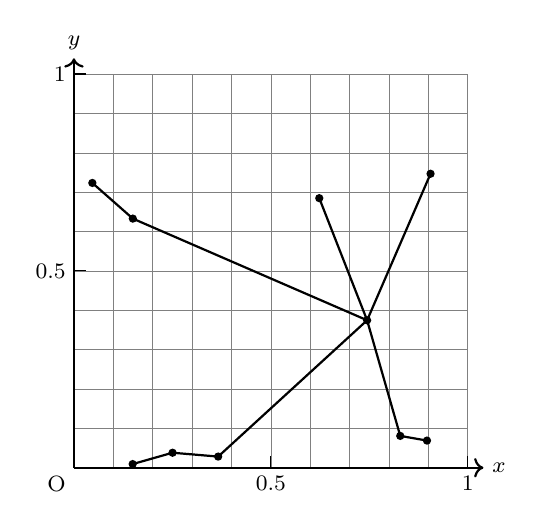
\begin{tikzpicture}[scale=0.5]\footnotesize
\draw[step=1cm,gray,very thin] (0,0) grid (10,10);
\foreach \x/\xtext in { 5/0.5, 10/1}
  \draw[black,xshift=\x cm] (0,.3) -- (0,0)
    node[below] {$\xtext$};
\foreach \y/\ytext in {5/0.5,10/1}
  \draw[black, yshift=\y cm] (.3,0) -- (0,0)
    node[left] {$\ytext$};
\draw[black] (0,0) node[anchor=north east] {O};
\draw[black,thick,->] (0, 0) -- (10.4, 0) node[right] {$x$};
\draw[black,thick,->] (0, 0) -- (0, 10.4) node[above] {$y$};

\coordinate (n0) at (6.2307871625908895,6.847027862484314);
\coordinate (n1) at (1.4908587845403831,9.344058188486937e-2);
\coordinate (n2) at (8.287496589039378,0.8087839284280984);
\coordinate (n3) at (3.662398504604587,0.2833983731779788);
\coordinate (n4) at (0.46715307814554796,7.233804012602063);
\coordinate (n5) at (9.057142532479283,7.467617781163527);
\coordinate (n6) at (7.44580515795162,3.7458151873056766);
\coordinate (n7) at (2.5041109412617235,0.3813699908645396);
\coordinate (n8) at (1.4952402484562444,6.327917885574969);
\coordinate (n9) at (8.966635336689189,0.6898816967621113);
\draw[thick] (n0) -- (n6);
\draw[thick] (n1) -- (n7);
\draw[thick] (n3) -- (n6);
\draw[thick] (n4) -- (n8);
\draw[thick] (n5) -- (n6);
\draw[thick] (n6) -- (n2);
\draw[thick] (n7) -- (n3);
\draw[thick] (n8) -- (n6);
\draw[thick] (n9) -- (n2);

\foreach \n in {n0,n1,n2,n3,n4,n5,n6,n7,n8,n9}
  \fill (\n) circle [radius=3pt];

\end{tikzpicture}
\end{subfigure}
\quad
\begin{subfigure}[t]{0.5\textwidth}
\centering
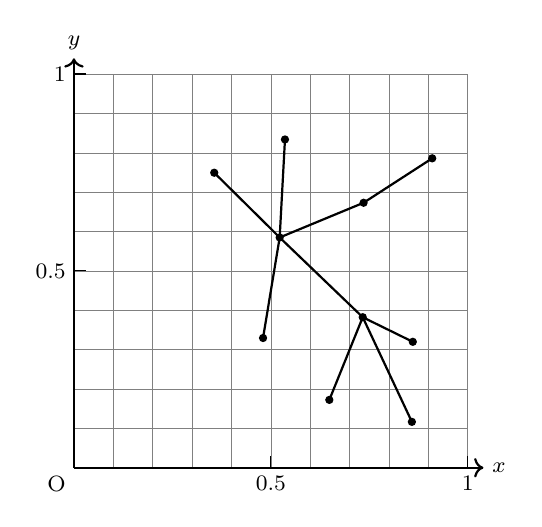
\begin{tikzpicture}[scale=0.5]\footnotesize
\draw[step=1cm,gray,very thin] (0,0) grid (10,10);
\foreach \x/\xtext in { 5/0.5, 10/1}
  \draw[black,xshift=\x cm] (0,.3) -- (0,0)
    node[below] {$\xtext$};
\foreach \y/\ytext in {5/0.5,10/1}
  \draw[black, yshift=\y cm] (.3,0) -- (0,0)
    node[left] {$\ytext$};
\draw[black] (0,0) node[anchor=north east] {O};
\draw[black,thick,->] (0, 0) -- (10.4, 0) node[right] {$x$};
\draw[black,thick,->] (0, 0) -- (0, 10.4) node[above] {$y$};

\coordinate (n0) at (6.486317401060322,1.7238949217908428);
\coordinate (n1) at (7.356328176128615,6.7307533977302025);
\coordinate (n2) at (3.5627260906386415,7.493578518706636);
\coordinate (n3) at (8.582933996984575,1.1655496682661926);
\coordinate (n4) at (5.35937147771363,8.338368157065618);
\coordinate (n5) at (5.224998480720355,5.848686799435092);
\coordinate (n6) at (4.8023010605002465,3.2954642049633076);
\coordinate (n7) at (7.334875634225844,3.82310788843208);
\coordinate (n8) at (8.606186458999954,3.198710520132577);
\coordinate (n9) at (9.099399064468583,7.859275597076669);
\draw[thick] (n0) -- (n7);
\draw[thick] (n2) -- (n5);
\draw[thick] (n3) -- (n7);
\draw[thick] (n4) -- (n5);
\draw[thick] (n5) -- (n1);
\draw[thick] (n6) -- (n5);
\draw[thick] (n7) -- (n5);
\draw[thick] (n8) -- (n7);
\draw[thick] (n9) -- (n1);
\foreach \n in {n0,n1,n2,n3,n4,n5,n6,n7,n8,n9}
  \fill (\n) circle [radius=3pt];

\end{tikzpicture}
\end{subfigure}
\caption{Examples of 10-node minimum pair distance trees for uniformly random 2-dimensional points in the unit square and euclidean weights between them.}
\label{fig:minPairDist}
\end{figure}

\paragraph{Approximated Mimimum Pair Distance}

Because calculating the actual minimum pair distance tree is impractical, we describe an algorithm that constructs a tree in $\mathcal{O}(n^3)$ time that tries to minimize pair distance as well as possible. Let $c_{G'}(u, v)$ denote the distance of the shortest path from $u$ to $v$ in a tree graph $G'=(V',E')$ of nodes $V'\subset V$ and edges $E'\subset E$. Then let $\mathcal{C}_{pairs}(G')$ denote the total distance between all pairs of nodes in $G'$.
\begin{equation}
\mathcal{C}_{pairs}(G') = \sum_{u,v\in V'}c_{G'}(u,v)
\end{equation}

The algorithm is based on the idea of connecting nodes one-by-one to the tree, in every step choosing the node and a connecting edge that minimizes the total pair distance. We do this efficiently by maintaining a data structure that allows querying the increase of total pair distance for a node and edge in constant time.

Let $V'$ be the set of nodes currently included in the tree. $V'$ gets initialized to $\{r\}$ where $r$ is an arbitrarily chosen node. Our data structure then encompasses an array $p:V'\to\mathbb{R}$, where $p(v)$ stores the total distance from node $v$ to all other nodes $V'\setminus\{v\}$ in the current tree. In addition, a two-dimensional array $s:(V',V')\to\mathbb{R}$ is needed, where $s(u,v)$ stores the shortest distance in the tree between nodes $u$ and $v$.
\begin{equation}
\begin{split}
s(u,v)=&c_{G'}(u,v)\\
p(u)=&\sum_{i\in V'}c_{G'}(i,u) \\
\end{split}
\end{equation}

Now if edge $(u,v)$ with $u\in V'$ and $v\in V\setminus V'$ were to get added to the tree to get $G''=G'\cup(\{v\}, \{(u,v)\})$, the total pair distance increases only by the new pairs from $v$ to all nodes in $V'$. With our data structure we can calculate this increase in constant time:
\begin{equation}
\begin{split}
& \mathcal{C}_{pairs}(G'')-\mathcal{C}_{pairs}(G') \\
=\;&\sum_{i\in V'}c_{G''}(i, v)+\sum_{i\in V'}c_{G''}(v, i)=2\sum_{i\in V'}c_{G''}(i, v) \\
=\;&2\sum_{i\in V'}\left(c_{G'}(i,u)+c(u,v)\right)=2\left(\sum_{i\in V'}c_{G'}(i,u)+|V'|\cdot c(u,v)\right) \\
=\;&2\left(p(u)+|V'|\cdot c(u,v)\right) \\
\end{split}
\end{equation}

In addition, we can update our data structure for the new edge $(u,v)$ in linear time:
\begin{itemize}
\item To set the total distance from $v$ to all other nodes is just the total distance to all other nodes from $u$, plus the new edge once for every node: $p(v)\gets p(u)+|V'|\cdot c(u,v)$
\item For all other nodes, $p$ needs to be increased by the shortest path to $v$, which is just the shortest path to $u$ plus the cost of the edge $(u,v)$: $p(i)\gets p(i)+s(i,u)+c(u,v)$ for all $i\in V'$
\item Also the shortest path from all nodes to $v$ gets initialized to the shortest path to $u$ plus the cost of the edge $(u,v)$: $s(i,v)\gets s(i,u)+c(u,v)$ for all $i\in V'$
\item Similarly the shortest path from $v$ to all nodes: $s(v,i)\gets c(v,u)+s(u,i)$ for all $i\in V'$
\end{itemize}

As a result, our algorithm looks as follows:
\begin{enumerate}
\item Set $V'=\{r\}$ for an arbitrary node $r\in V$ and initialize $p(r)=0$ and $s(r,r)=0$
\item Add the edge $(u,v)$ ($u\in V'$ and $v\in V\setminus V'$) which increases the total pair distance by the minimum to the resulting tree
\label{approxStep}
\item Update $p$ and $s$ according to the new edge
\item Unless $V'=V$, go to step \ref{approxStep}
\end{enumerate}

Because the tree gets one more node in every iteration, the sequence of the number of edges between tree and non-tree nodes is $1n,2(n-1),3(n-2),\dots,(n-1)2,n1$. Every iteration therefore takes $\mathcal{O}(n^2)$ to find the best edge and an additional $\mathcal{O}(n)$ to update the data structure. The total complexity of this algorithm is therefore $\mathcal{O}(n\cdot(n^2+n))=\mathcal{O}(n^3)$.

\TODO{Go into how good this actually is?}

\chapter{Implementation Notes}

As part of this thesis, a Haskell library for writing and testing Arvy algorithms was created, accessible at \url{https://github.com/infinisil/arvy}. In this chapter we explain some key design decisions that went into it. With Haskell's advanced type system it's possible to guarantee correctness of all Arvy heuristics declared with this library. Needless to say, this chapter is more technical than the others and advanced Haskell knowledge is required to fully understand it.

\section{Request Path abstraction}

An Arvy algorithm is only correct if and only if nodes can only set their new parent to nodes that were previously visited on the request path. With each node being referenced as an integer, this would be a problem, because a node $a_{n+1}$ could simply set $parent(a_{n+1})=0$ even though it might be the case that $0\notin\{a_0,\dots,a_n\}$ which would make the algorithm incorrect. So instead of representing nodes as integers, we represent them as some arbitrary type with certain capabilities that reflect them being part of the request path.

One such trivial capability we'll need is that once we have some node index, we can forward that value via messages to other nodes. This makes sense since some node $a_{n+1}$ can't know about $\{a_0,\dots,a_n\}$ unless these nodes somehow forwarded their own values along with the messages. In Haskell, this forwarding can be represented as a typeclass on two types $i_a$ and $i_b$, stating that if you have a value of $i_a$ you can get a value of $i_b$. We can implement this typeclass trivially for all types that are equal, since forwarding will then be the identity.

\begin{minted}{haskell}
-- | A class for node indices that can be forwarded between nodes
class Forwardable ia ib where
  forward :: ia -> ib

-- | All equivalent types can be trivially forwarded
instance Forwardable i i where
  forward = id
\end{minted}

Now we need to somehow encode a request path in a type. In such a request path the important constraint is that messages are only sent in one direction, meaning node indices can only be forwarded in one direction as well. Looking at it from a single node in the request path, we can forward from its predecessor to the current node and from the current node to its successor. Encoding this as a typeclass leaves us with the following for representing a node (index).

\begin{minted}{haskell}
class ( Forwardable (Pred i) i
      , Forwardable i (Succ i)
      ) => NodeIndex i where
  -- The type representing the previous node
  type Pred i :: *
  -- The type representing the successor node
  type Succ i :: *
\end{minted}

Now of course defining different types for every node along the request path is impossible, this is only used to prove correctness. So for the implementation, we can use integers to represent all nodes.

\begin{minted}{haskell}
type Node = Int

instance NodeIndex Node where
  -- Predecessors and successors in the request path are
  -- all nodes represented by integers as well
  type Pred Node = Node
  type Succ Node = Node
\end{minted}

\section{Arvy Heuristic abstraction}

The most important part of defining an Arvy algorithm is the heuristic it uses to decide the new node parent. We extend this to the notion of a behavior, which includes not only the new parents, but also how it gets decided what a request message looks like, how the initial message is generated, and what the final node receiving the message does. In fact each node on the request path should be allowed to run arbitrary code when they do the processing.

For representing computations we use the relatively new effect library \href{https://hackage.haskell.org/package/polysemy}{Polysemy}. In this library an computation is described with $\texttt{Sem r a}$ where $\texttt{r}$ represents the possible effects it can have and $\texttt{a}$ being the result of the computation. With this said, the main type for defining an Arvy algorithm is defined as follows.

\begin{minted}{haskell}
{- |
An Arvy heuristic for a dynamic algorithm.
- @i@ is the node index type
- @msg :: * -> *@ is the type of request messages passed between nodes,
  parametrized by the node index type for allowing messages to forward
  node indices
- @r@ is the effects the algorithm runs in, which can include effects
  parametrized by @i@ in order to allow effects dependent on indices
-}
data ArvyBehavior i msg r = ArvyBehavior
  { arvyMakeRequest :: i -> Succ i -> Sem r (msg i)
  -- ^ What message the node making the request should send to its parent
  , arvyForwardRequest :: msg (Pred i) -> i -> Succ i -> Sem r (Pred i, msg i)
  -- ^ What parent an intermediate node should select when receiving
  -- a message, and what message to forward to its parent
  , arvyReceiveRequest :: msg (Pred i) -> i -> Sem r (Pred i)
  -- ^ What parent the last node should select when receiving a message
  }
\end{minted}

This succinct-yet-complicated type includes a lot of information. The type signature of the $\texttt{arvyForwardRequest}$ function in particular is the most interesting.

For one it says that an intermediate node receives a message $\texttt{msg (Pred i)}$ that can include node indices of nodes that were predecessors to the current node. It then needs to return a value of $\texttt{Pred i}$, which represents the new parent for the node. With how node indices are defined in the previous section, the only possible values to return are ones received from the message. This means to select a new parent, nodes have to decode the message which will contain node indices given by past nodes, then return one of them.

In addition, the function receives values $\texttt{i}$ and $\texttt{Succ i}$ representing the current node index and the current nodes parent respectively. In addition to the new parent node to select, the function also needs to return a $\texttt{msg i}$ representing the message to be forwarded. The $\texttt{msg}$ type being parametrized by $\texttt{i}$ enforces that this message can only contain node indices to previous nodes (since all previous node indices $\texttt{Pred i}$ can be forwarded to $\texttt{i}$) or the current node (which is of type $\texttt{i}$ already). $\texttt{Succ i}$ however can't be sent in the message because there's no way to convert it to type $\texttt{i}$.

Functions $\texttt{arvyMakeRequest}$ and $\texttt{arvyReceiveRequest}$ are special cases of $\texttt{arvyForwardRequest}$. The former of which is special in that a node making a request does not receive any message and it doesn't need to select a new parent since it becomes the root. The latter of which is special in that the final root node receiving the request doesn't have a parent and doesn't need to forward a message.

\chapter{Results}

Should include
\begin{itemize}
\item Resulting plots of interesting evaluations
\item Show how to reproduce the results including parameters
\end{itemize}

What are the results?
\begin{itemize}
\item Ivy is better than the best arrow for cliques with node counts only <5
\item For uniformly random requests, the best star is a very good tree
\item 
\end{itemize}

\section{Ivy is better than Arrow for cliques of less than 5 nodes}
\label{result:clique}

\chapter{Summary}


\bibliographystyle{IEEEtran}
\bibliography{references}

%\appendix
%\chapter{First Appendix Chapter Title}

\end{document}
